\documentclass[11pt]{article}


\usepackage{graphicx}
\usepackage[margin=1in]{geometry}
\usepackage{xfrac}
\usepackage{amsmath}
\usepackage{amssymb}

\graphicspath{{./img/}}
\DeclareGraphicsExtensions{.pdf}

\newcommand{\bibfile}{refs.bib}

\newcommand{\kt}{k_B T}
\newcommand{\expect}[1]{\langle #1 \rangle}
\newcommand{\One}{\hat{1}}


\begin{document}


\section{Background}

\subsection{Marcus Hopping}

Starting with Fermi's Golden Rule, the transfer rate between some initial and final state can be found \cite{jortner76, lin02, nan09}:
\begin{equation}
\nu_{if} = \frac{|t_{if}|^2}{\hbar^2} \int_0^\infty dt \cos \left(\sum_j S_j\sin \omega_jt \right) e^{-\sum_j S_j (2n_j+1)(1-\cos \omega_jt)},
\end{equation}
where $t_{if}$ is the transfer integral and $S_j = \sfrac{\lambda_j}{\hbar\omega_j}$ and $n_j = [e^{\sfrac{\hbar\omega_j}{\kt}}-1]^{-1}$ are the Huang-Rhys factor and population of the $j^{th}$ normal vibrational mode. In either the strong coupling limit ($\sum_j S_j \gg 1$) or the high temperature limit ($\kt \gg \hbar \omega_j$ for dominant vibration modes), this expression simplifies to \cite{shuai12}
\begin{equation}
\nu_{if} = \frac{|t_{if}|^2}{\hbar^2} \sqrt{\frac{2\pi}{\sum_j S_j \omega_j^2(2n_j+1)}} e^{-\frac{(\omega_{if}+\sum_j S_j \omega_j)^2}{2\sum_j S_j\omega_j^2(2n_j+1)}}.
\end{equation}
In the high-temperature limit, this reduces to the Marcus hopping rate equation \cite{marcus93}:
\begin{equation}
\nu_{if} = \frac{|t_{if}|^2}{\hbar} \sqrt{\frac{\pi}{\lambda \kt}} \: e^{-\frac{(\Delta G_{if}+\lambda)^2}{4\lambda \kt}},
\end{equation}
with $\Delta G_{if} = \hbar \omega_{if}$ the change in Gibbs free energy between the two configurations and $\lambda = \sum_j S_j \hbar \omega_j$ the so-called "reorganization energy" associated with effort needed to undergo the state transition.


\subsection{Dangling Bond Hopping Model}
%
\begin{figure}[h!]
\centering
 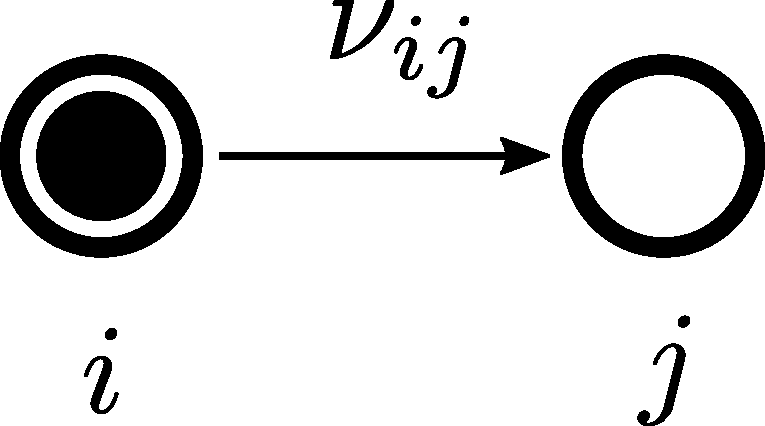
\includegraphics[width=.2\textwidth]{2db-nu}
 \caption{A single electron hops between two DBs with a transfer rate given by Marcus Theory.}
 \label{fig:2db-nu}
\end{figure}
%
Consider two dangling bonds which share an electron. According to Marcus Theory, the electron hops between the two DBs with a transfer rate:
\begin{equation}
\nu_{ij} = \frac{|t_{ij}|^2}{\hbar} \sqrt{\frac{\pi}{\lambda k_B T}} e^{-\frac{(\Delta G_{ij} + \lambda)^2}{4\lambda \kt}}
\end{equation}
where
\begin{align*}
t_{ij} &: \text{electron transfer integral}\\
\lambda &: \text{reorganization energy; self-trapping energy}\\
\Delta G_{ij} &: \text{change in Gibbs free energy for the electron transfer}
\end{align*}
The transfer integrals arise from the DB orbital overlap and can be assumed to be a function only of the DB arrangement and fixed throughout the surface simulation. The reorganization energy is a fixed property of the lattice and is identical for all DBs.
\begin{figure}
\centering
 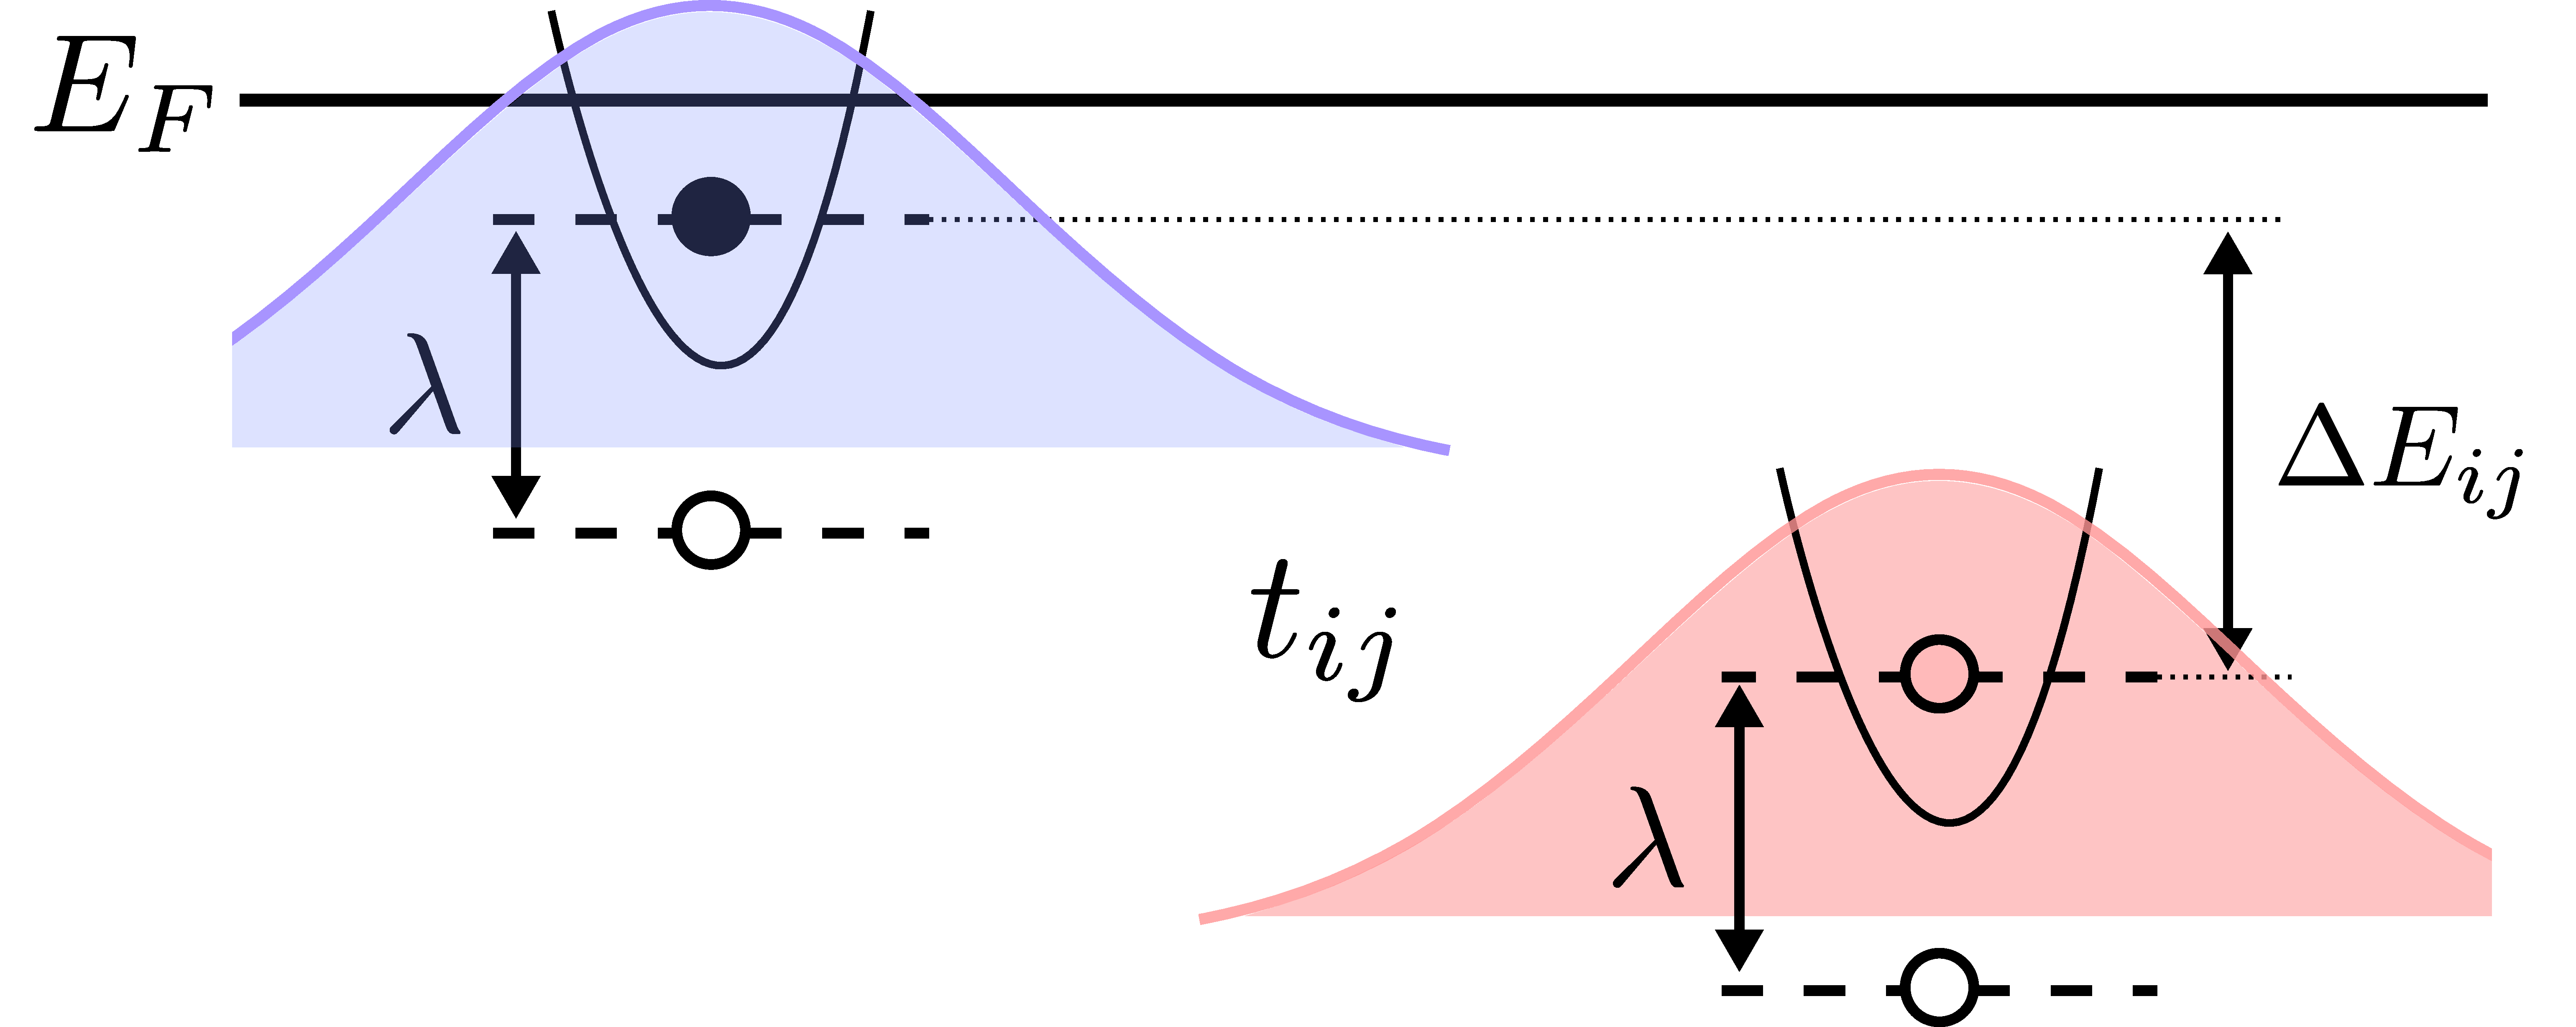
\includegraphics[width=.7\textwidth]{2db-landscape}
 \caption{Each DB is modelled as a well with a single bound state. When a DB contains an electron, that electron is self-trapped with a given energy $\lambda$. The energy level of each well is determined by the local potential at that well arising both from external fields such as those from the tip and from Coulombic interactions between occupying electrons. The wavefunction overlap between the wells gives the transfer integrals.}
 \label{fig:2db-landscape}
\end{figure}
Each of the DBs is identical so the change in Gibbs free energy arises only from the occupation energy of each DB: $\Delta G_{ij} \approx \Delta E_{ij}$. The energy of a charge configuration $\vec{n}$ is of the form
\begin{equation}
E(\vec{n}) = -\sum_i U_i n_i + \frac{1}{2} \sum_{<i,j>} V_{ij}n_in_j = -\vec{U}^T\vec{n} + \frac{1}{2}\vec{n}^T V \vec{n}
\end{equation}
where $n_i$ is the number of electrons at the $i^{th}$ site, $U_i$ is the local potential due to external fields such as those from thetip, and $V_{ij}$ is the strength of the Coulombic interaction between each site. We approximate any potential Debye screening by using an interaction of the form
\begin{equation}
V_{ij} = \frac{q}{4\pi\epsilon r_{ij}}e^{\sfrac{-r_{ij}}{\lambda_D}}
\end{equation}
with $r_{ij}$ the distance between DBs and $\lambda_D$ the Debye length.

\subsection{Hopping Intervals}

For a given hopping rate $\nu$, we should expect a hop to occur after $\expect{\tau} = \nu^{-1}$ seconds, where $\tau$ is the hopping interval. If $\nu$ is fixed, $\tau$ is an exponential random variable with probability $P(\tau \leq t) = 1-e^{-\nu t}$. We can interpret the transfer dynamics in two ways:
\begin{enumerate}
 \item a hop is attempted after some $\tau$ seconds with $P(\tau \leq t) = 1-e^{-\nu t}$.
 \item a hop is attempted after some $\tau_0$ "ticks" with $P(\tau_0 \leq t) = 1-e^{-t}$ and a "tick rate" of $\nu$ ticks per second.
\end{enumerate}
This tick rate picture is convenient as it naturally leads to the behaviour for an electron among multiple DBs. Each possible hopping destination contributes $\nu_{ij}$ to the rate at which the electron "leaks" out of its current DB. Therefore, a hop occurs after $\tau_0$ ticks with the tick rate given as $\nu_i = \sum_j \nu_{ij}$. Further, the $\nu_{ij}$ can be time varying without any challenge (see Appendix \ref{app:tickrate}). We refer to $\tau_0$ as the \emph{lifetime} of a charge.

\subsection{Marcus-Boltzmann Distribution}

After $\tau$ seconds, an electron hops from site $i$ to some target $j$. The probability of hopping to $j$ is proportional to $\nu_{ij}$:
\begin{equation}
p_{ij} = \alpha \nu_{ij} = \frac{\nu_{ij}}{\sum_k \nu_{ik}}
\end{equation}
The form of this distribution has similar properties to the Boltzmann distribution. Namely, the hopping probability is highly affected by the resulting change in energy. For that reason, this distribution will be referred to as the Marcus-Boltzmann distribution:
\[
p_{ij} = \frac{|t_{ij}|^2 e^{-\frac{(\Delta E_{ij}+\lambda)^2}{4\lambda \kt}}}{\sum_k |t_{ik}|^2 e^{-\frac{(\Delta E_{ik}+\lambda)^2}{4\lambda \kt}}}
\]

\emph{Question: is this necessarily true? For time varying $\nu_{ij}$ it might make more sense that the probability be something more like}
\[
p_{ij} = \frac{\int_0^\tau \nu_{ij}(t) dt}{\sum_k \int_0^\tau \nu_{ik}(t) dt}
\]
\emph{as this would give the weighted accumulated charge leakage to each possible hopping target rather than using only the instantaneous rates. However, this might result in charges hopping to sites which recently became unfavourable due to other hopping events. Also there are issues: what if most of the charge leakage (consumption of $\tau_0$) was to a DB which was later occupied and hence no longer available? }

\section{Numerical Details}

Recall that the energy associated with a charge configuration is given as
\[
E(\vec{n}) = -\vec{U}^T\vec{n} + \frac{1}{2}\vec{n}^T V \vec{n}.
\]
An electron now tunnels from site $i$ to $j$: $\delta \vec{n} = \vec{n}' - \vec{n} = \hat{e}_j - \hat{e}_i$. Assuming $\vec{U}$ is independent of the charge state, the change in energy is computed as
\begin{align*}
\Delta E_{ij} = E(\vec{n}') - E(\vec{n}) = -\vec{U}^T \delta \vec{n}+ \frac{1}{2} \left[\vec{n}'^T V \vec{n}' - \vec{n}^T V \vec{n} \right] = -[\vec{U} - V\vec{n}]^T\delta \vec{n} - V_{ij}.
\end{align*}
If we define $\vec{\epsilon} = \vec{U} - V\vec{n}$, we obtain the convenient expression:
\begin{equation}
\Delta E = \hat{\epsilon} \otimes \One^T - \One \otimes \hat{\epsilon}^T - V
\end{equation}
where $\Delta E$ is the matrix of all possible energy changes for the current charge state. Note that either Python or MATLAB will do the broadcasting for free so this is simply $\Delta E = \vec{\epsilon} - \vec{\epsilon}^T - V$. One important efficiency note here is that for a charge state with $N$ electrons among $M$ DBs, there are only $N$ rows (hopping sources) and $M-N$ columns (hopping targets) that are relevant to the calculations. If we slice $\vec{\epsilon}$ and $V$ appropriately, we only ever have to deal with a $\Delta E$ of size $N \times (M-N)$.




\section{Current Questions}

\subsection{Tip Model}

The tip induces an effective change in the local potentials at each site. This potential is a function of the current charge configuration and so cannot simply be considered an additional term in $\vec{U}$ like other external fields. There is no real obstacle to simply extending the interpretation of $\vec{U}$. We can generalise the $\Delta E_{ij}$ equation as follows:
\begin{equation}
\Delta E_{ij} = -[\vec{U}' -V\vec{n}]^T \delta \vec{n} - V_{ij} - \Delta \vec{U}^T \vec{n}
\end{equation}
where $\vec{U}' = \vec{U}(\vec{n}')$ is the vector of local potentials after the hop, and $\Delta \vec{U} = \vec{U}' - \vec{U}$. For every $i$ and $j$ there is new $\vec{U}'$ and so we can't do any additional tricks without more information: i.e. how much can the tip model be parametrized, how many states do we expect to see near equilibrium (store tip influence for each state in a look-up table), etc.

\subsection{Population}

The current implementation of the Marcus simulator fixes the number of electrons. Nothing regarding the Fermi level is considered. One simple approach which could be easily implemented is to add an additional hopping channel to/from a reservoir. The effective potential experiencde at each DB is given as
\begin{equation}
\vec{U}_{eff} = \vec{U} - V \vec{n}
\end{equation}
This is of course equal to $\vec{\epsilon}$ from before. This is a measure of the absolute energy of the bound state of each well. There is a tranfer rate from all occupied DBs \textbf{to} the reservoir and \textbf{from} the reservoir to all empty DBs. This rate is a function of $\vec{U}_{eff}$. It is just a matter of finding the right parameters to match experiment.






\clearpage
\appendix

\section{Validation of the Tick-Rate Interpretation}
\label{app:tickrate}

Given some time varying transfer rate $\nu(t)$, the probability of a hopping event occuring in some small time dt is given by 
\begin{equation}
p(t) = \nu(t) dt.
\end{equation}
The hopping interval, i.e. the time until the first hopping event, is found to have probability
\begin{equation}
P(\tau \leq t) = 1-e^{-\int_0^t \nu(t')dt'}.
\end{equation}
Suppose we generate some exponential random variable $\tau_0$ according to
\begin{equation}
P(\tau_0 \leq t) = 1-e^{-t}
\end{equation}
and at each instant in time, we decrement $\tau_0$ by $\nu(t)dt$. The time, $\tau$, until $\tau_0$ is depleted is given implicitely as
\begin{equation}
\tau_0 = \int_0^\tau \nu(t) dt.
\end{equation}
We are interested in the quantity $P(\tau \leq t)$. If we assume $\nu(t)>0$ then $\tau \leq t$ is equivalent to $\int_0^\tau \nu(t') dt' \leq \int_0^t \nu(t')dt'$. It follows then that
\begin{equation}
P(\tau \leq t) = P\left( \tau_0 \leq \int_0^t \nu(t')dt' \right) = 1-e^{-\int_0^t \nu(t')dt'}
\end{equation}
So $\tau$ has exactly the correct statistics. Note that on generating $\tau_0$ we knew nothing about the future values of $\nu(t)$. By consuming $\tau_0$ at the current $\nu(t)$, we effectively have generated the waiting time consistent with the future transfer rates. Therefore any change to the future charge state (and transfer rates) is automatically accounted for.


%\section{Detailed Balance}
%\label{app:balance}
%In equilibrium, detailed balance is achieved when the incoming and outgoing charge are equal:
%\begin{equation}
%\sum_i n_i \nu_{ik} = n_k \sum_i \nu_{ki} \quad \forall k
%\end{equation}
%Of course, the transfer rates are themselves functions of the charge state and not constants so we must be careful about their value at equilibrium.
%Consider the ratio of transfer rates between two sites $i$, $j$.
%\begin{equation}
%\frac{\nu_{ij}}{\nu_{ji}} = \frac{|t_{ij}|^2}{|t_{ji}|^2} e^{-\frac{1}{4\lambda \kt} \left[ (\Delta G_{ij} + \lambda)^2 - (\Delta G_{ji} + \lambda)^2 \right]} = e^{-\sfrac{\Delta G_{ij}}{\kt}}
%\end{equation}
%where we have only assumed that $|t_{ij}| = |t_{ji}|$. 
%Hence, equilibrium flow of charge is governed by Gibbs factor weighted rates.


\bibliographystyle{ieeetr}
\bibliography{\bibfile}

\end{document}